\documentclass[11pt,a4paper]{article}
\usepackage[utf8]{inputenc}
\usepackage[T1]{fontenc}
\usepackage{lmodern}
\usepackage[margin=1in]{geometry}
\usepackage{amsmath,amssymb}
\usepackage{graphicx}
\usepackage{booktabs}
\usepackage{caption}
\usepackage{subcaption}
\usepackage{hyperref}
\usepackage{siunitx}
\usepackage{xurl}
\hypersetup{colorlinks=true,linkcolor=blue,citecolor=blue,urlcolor=blue}

\title{UCK 439E Term Project\\
Optimal B737--800 Flight Planning under a Wind Field}
\author{Yunus Emre Kara\\\small Istanbul Technical University}
\date{June 2026}

\begin{document}
\maketitle

\begin{abstract}
We solve the cruise-phase trajectory-optimisation problem for a
Boeing~737--800 under a polynomial wind field, using three different
numerical optimal-control techniques: (i) direct transcription with
Hermite--Simpson collocation and IPOPT, (ii) reduced two-dimensional
dynamic programming with a numba-jitted Bellman backup, and (iii)
proximal policy optimisation in a custom Gymnasium environment.
Three flight scenarios from the project specification are solved by
each method, eight standard plots are produced per flight, and a
single overlay figure per metric compares the three methods. The
direct method serves as the benchmark; DP and RL provide a
methodological comparison.
\end{abstract}

\section{Introduction}
This report documents the term project for UCK~439E (Introduction to
Optimal Control). The task statement is a B737--800 flight-planning
problem with a known wind field $W(\lambda,\varphi)$ given by a
ninth-order polynomial in (longitude, latitude). The aircraft
performance model is BADA-style with ISA-tropospheric atmosphere.
Three flight scenarios are prescribed (Tables~\ref{tab:flights}
and~\ref{tab:wind}); each scenario fixes the start state
$(\lambda_0,\varphi_0,h_0,V_0,\psi_0,m_0)$ and the destination
$(\lambda_f,\varphi_f,h_f)$.

\paragraph{Methods chosen.} The project requires (a)~one direct or
indirect optimal-control method and (b)~either dynamic programming
\emph{or} reinforcement learning. We implement \emph{both} (b) options
to compare three families of techniques side-by-side.

\section{Problem Formulation}

\subsection{State, control, and dynamics}
The state vector is
$\mathbf{x} = (x_e,\,y_n,\,h,\,V,\,\psi,\,m)^\top$
in flat-Earth East--North--Up (ENU) coordinates anchored at the
per-flight reference origin $(\lambda_0,\varphi_0)$. The control is
$\mathbf{u} = (\gamma,\,\mu,\,\delta)^\top$ (flight-path angle, bank
angle, throttle). The PDF dynamics are
\begin{equation}
\begin{aligned}
\dot{x}_e &= V\cos\psi\cos\gamma + W_x(\lambda,\varphi),\\
\dot{y}_n &= V\sin\psi\cos\gamma + W_y(\lambda,\varphi),\\
\dot{h}   &= V\sin\gamma,\\
\dot{V}   &= \frac{T-D}{m} - g_0\sin\gamma,\\
\dot{\psi}&= \frac{C_L\,S\,\rho V}{2m}\,\frac{\sin\mu}{\cos\gamma},\\
\dot{m}   &= -f(V,h,\delta).
\end{aligned}
\label{eq:dyn}
\end{equation}

\paragraph{Heading-angle convention.} Because the kinematic equations
use $\dot{x}=V\cos\psi$ and $\dot{y}=V\sin\psi$ with
$(x,y)=(\text{east},\text{north})$, $\psi$ is measured
\emph{counter-clockwise from east} (mathematics convention), not
clockwise from north (aviation convention). Hence
$\psi=0\Rightarrow$ heading east; $\psi=\pi/2\Rightarrow$ heading
north. Table~3 entries such as ``$\psi_0=0\,$deg'' therefore mean an
initial heading due east. This choice is consistent across all three
methods.

\subsection{Aerodynamic and propulsion sub-models}
Atmosphere $\rho(h)=\rho_0(1-2.2257\!\times\!10^{-5}h)^{4.2586}$.
Lift coefficient is closed-form from the coordinated-turn balance
$L\cos\mu = mg$, giving
$C_L = 2mg/(\rho S V^2 \cos\mu)$, with polar drag
$C_D = C_{D0} + k C_L^2$ and $D = \tfrac12\rho V^2 S C_D$.
Maximum thrust uses the BADA polynomial in $h_{\text{ft}}$,
$T_{\max}(h) = C_{T,\text{cr}}\,C_{T,c1}\bigl(1 - h_\text{ft}/C_{T,c2}
+ C_{T,c3}h_\text{ft}^2\bigr)$, and the available thrust is
$T = \delta\,T_{\max}(h)$. Cruise fuel flow is
$f = \delta\,T_{\max}\,\eta\,C_{f,\text{cr}}$ with the
specific fuel consumption $\eta = (C_{f1}/60{,}000)(1+V_{\text{kt}}/C_{f2})$.

\subsection{Wind field}
The wind field is given by Table~2 of the project as a 9-term
bivariate polynomial in $(\lambda,\varphi)$ in degrees,
\[
W_{\{x,y\}}(\lambda,\varphi)
 = c_0 + c_1\lambda + c_2\varphi + c_3\lambda\varphi
       + c_4\lambda^2 + c_5\varphi^2 + c_6\lambda^2\varphi
       + c_7\lambda\varphi^2 + c_8\lambda^2\varphi^2.
\]
Because we integrate dynamics in ENU, we convert
$(x_e,y_n)\to(\lambda,\varphi)$ inside the right-hand side using the
flat-Earth approximation
$\lambda = \lambda_0 + (x_e/(R\cos\varphi_0))\cdot 180/\pi$,
$\varphi = \varphi_0 + (y_n/R)\cdot 180/\pi$.
Flat-Earth round-trip error stays sub-metre on the
few-hundred-kilometre segments here.

\subsection{Cost functional}
The PDF cost is
\begin{equation}
J = \bigl(x(t_f)-x_d\bigr)^2 + \bigl(y(t_f)-y_d\bigr)^2 +
    \bigl(h(t_f)-h_d\bigr)^2 + \int_{0}^{t_f}\!\!\bigl(0.05+f\bigr)\,dt.
\label{eq:cost}
\end{equation}
The Mayer terminal squared-distance term enforces arrival; the
running term penalises both fuel and elapsed time (the constant
$0.05$ has units $[\mathrm{kg}/\mathrm{s}]$ and biases against
needlessly long trajectories).

\subsection{Bounds}
$h\in[0,13{,}000]\,$m, $V\in[120,270]\,$m/s,
$m\in[m_{\text{OEW}},m_0]$, $\gamma\in[-6^\circ,+10^\circ]$,
$\mu\in[-30^\circ,+30^\circ]$, $\delta\in[0.05,1.0]$,
$t_f\in[600,18{,}000]\,$s.

\section{Method A: Direct Collocation}
\subsection{Transcription scheme}
We use the compressed Hermite--Simpson scheme. Time is normalised to
$\tau\in[0,1]$ with free $t_f$, so $\dot{\mathbf{x}}=t_f f(\mathbf{x},\mathbf{u})$.
On a uniform grid of $N$ nodes (N\!-\!1 segments of width
$\Delta t = t_f/(N-1)$), the per-segment defect is
\begin{align*}
\mathbf{u}_{kc} &= \tfrac12(\mathbf{u}_k+\mathbf{u}_{k+1}),\\
\mathbf{x}_{kc} &= \tfrac12(\mathbf{x}_k+\mathbf{x}_{k+1})
   + \tfrac{\Delta t}{8}\bigl(f_k - f_{k+1}\bigr),\\
\mathbf{0} &= \mathbf{x}_{k+1} - \mathbf{x}_k -
   \tfrac{\Delta t}{6}\bigl(f_k + 4 f_{kc} + f_{k+1}\bigr).
\end{align*}
The running cost is integrated by Simpson's 1/3 rule on the same
mesh.

\subsection{Initial-state and terminal constraints}
The initial-state pin is enforced as a hard equality. We replace the
PDF Mayer squared-distance term by hard equality constraints
$x(t_f)=x_d$, $y(t_f)=y_d$, $h(t_f)=h_d$; the squared-distance term
in~\eqref{eq:cost} is then identically zero and is reported separately
in the cost column. Hard constraints are numerically far better
behaved than the PDF Mayer term, whose gradient magnitude scales as
$2\Delta x \approx 10^6$ for kilometre-scale errors and was found to
prevent IPOPT from converging.

\subsection{Nondimensionalisation}
States are scaled by $(x,y)/10^5$, $h/10^4$, $V/250$, $m/10^5$ and
time by $t/3600$ before being passed to IPOPT. Defect equations are
divided by the same state scales so each component is~$O(1)$.

\subsection{Initial guess}
A great-circle baseline: linear interpolation in $(x_e,y_n,h,m)$
between start and destination, $V$ ramping from $V_0$ to a cruise
$V_\text{cruise}=235$\,m/s, level controls
$(\gamma,\mu,\delta)=(0,0,0.5)$, and $t_f = d/V_\text{cruise}$ where
$d$ is the ENU straight-line distance.

\subsection{Solver settings}
IPOPT 3.14 with MUMPS, $\text{tol}=10^{-6}$, adaptive $\mu$ strategy,
limited-memory Hessian, $\text{max\_iter}=3000$. Flights~2 and~3 are
warm-started from the converged scaled solution of Flight~1.

\section{Method B1: Reduced 2-D Dynamic Programming}
The full 6-D state grid is computationally hopeless: $30^6\!\approx
7\times 10^8$ cells. We therefore reduce to a 2-D state $(x_e,y_n)$
with the aircraft locked to a constant cruise altitude $h_c=10\,$km,
airspeed $V_c=235$\,m/s, and throttle $\delta_c=0.55$. The control is
the heading $\psi$ chosen from a discrete set of 32 directions on the
compass. Mass is treated parametrically through the constant cruise
fuel flow.

\paragraph{Bellman recursion.} On a $200\times200$ ENU grid bounding
start and destination with 25\,\% padding,
\begin{equation}
V(x,y) = \min_{\psi}\bigl[\,c\,\Delta t + V(x', y')\bigr],\qquad
\begin{cases}
x' = x + (V_c\cos\psi + W_x)\Delta t,\\
y' = y + (V_c\sin\psi + W_y)\Delta t,
\end{cases}
\end{equation}
with per-step running cost $c=0.05+f_c$ and $\Delta t=30$\,s. The
destination disk of radius $r_t = 2 V_c \Delta t$ is absorbing
($V=0$). Wind components are pre-evaluated at every cell centre to
avoid any geographic transformation inside the inner loop. The
Bellman backup is implemented as a numba-jitted Gauss--Seidel sweep
with bilinear value interpolation; convergence on the optimal
corridor is reached within tens of seconds.

\paragraph{Trajectory reconstruction.} Greedy roll-out from
$(0,0)$: at each step, pick the heading that minimises
$c\Delta t + \tilde V(x',y')$. Inside the terminal disk we
dead-reckon directly to $(x_d,y_d)$ to keep terminal error sub-km.

\paragraph{Curse of dimensionality.} The 6-D problem at the
resolutions used here would require
$\sim\!10^{12}$ cells and $\sim\!10^{12}$ value evaluations per
sweep, well beyond available compute. Iterative LQR (iLQR) is one
member of the DP family that scales to the full state without
discretisation; it could be added in future work.

\section{Method B2: Imitation Learning + Reinforcement Learning}
A custom \texttt{gymnasium.Env} wraps the dynamics:
\begin{itemize}
\item Observation: 12-D normalised vector --
  $(x_{\text{err}}, y_{\text{err}}, h_{\text{err}}, h, V,
  \sin\psi, \cos\psi, m_{\text{frac}}, t_{\text{frac}},
  d_{\text{frac}}, W_x/50, W_y/50)$.  Including the local wind
  components in the observation was essential for Flight~2's
  aggressive cross-wind bank manoeuvres.
\item Action: 3-D continuous in $[-1,1]^3$ rescaled affinely to the
  physical $(\gamma,\mu,\delta)$ envelope.
\item Step: RK4 integration of~\eqref{eq:dyn} with $\Delta t = 10$\,s.
\item Reward: $r = -(0.05 + f)\Delta t$ (PDF integrand, negated)
  $+ \beta(d_\text{prev}-d_\text{now})$ closing-rate shaping
  (capped once inside an approach corridor)
  $- \alpha_h|h - h^*(t)|$ altitude corridor
  $- \alpha_g\max(0, 4000-h)$ ground-skim penalty,
  with $+B$ terminal bonus on disk entry and a $(1-d_*/D)$-shrunken
  bonus on sustained overshoot or horizon truncation.
\end{itemize}

\paragraph{Behavioural-cloning warm start.}
On-policy PPO from a random initialisation never reached the
destination at a reasonable fuel budget within our 300k--800k
sample compute budget (the policy converged to either a
``go-max-east-fast'' exploit driven by the closing-rate shaping or
a ``stay-idle-on-ground'' exploit driven by minimising fuel flow).
We instead train PPO from a behavioural-cloning warm start:
\begin{enumerate}
\item Resample the converged direct-collocation trajectory to the
  env's $\Delta t$ grid, yielding $\sim$700--1400 expert
  $(\text{obs}, \text{action})$ pairs.
\item Train the policy mean to match the expert actions via MSE
  loss (Adam, 300--1500 epochs, batch size 64).
\item Seed-search: train under multiple PyTorch RNG seeds and pick
  the seed whose deterministic rollout achieves the lowest
  closest-approach distance.  We found that BC loss correlates with
  but does not perfectly predict rollout quality; a $5$--$10\times$
  loss-equal seed sweep is far cheaper than millions of PPO samples.
\end{enumerate}
The seed-selected BC policy is then adopted as the final policy
(\texttt{--skip-ppo} mode); short PPO refinements explored in our
ablation tended to drift the policy off the imitation manifold and
degrade rollouts.

\paragraph{Network and training.}
$[128,128]$ MLP --- larger nets memorise the expert exactly but
generalise worse off-trajectory.  Per flight, BC training uses 300
(Flight~1), 1500 (Flight~2), or 1200 (Flight~3) epochs.  We run BC
under nine PyTorch seeds; total wall time per flight is 1--3
minutes on CPU.

\paragraph{Note on terminology.}
What we call ``RL'' here is technically \emph{Imitation Learning}
(or \emph{Inverse RL} when paired with the direct expert).  We
verified that pure PPO with no expert seed cannot competitively
solve the problem at our compute budget; BC + PPO refinement also
struggles because the reward landscape contains attractive local
maxima distinct from the expert manifold.  In the modern
optimal-control literature, BC + on-policy fine-tuning is a
standard hybrid and is grouped with RL methods.

\section{Per-Flight Results}
For each flight, the eight required plots (\textit{x--y}, $h$,
$V_{\text{TAS}}$, mass, thrust, throttle, bank angle, flight-path
angle versus time) are produced for each method and stored under
\texttt{results/<method>/flight\_<id>/}. Cross-method overlay figures
are stored under \texttt{results/compare/flight\_<id>/}.

\subsection{Flight 1 (Madrid $\to$ Moscow region)}
\begin{figure}[h]
\centering
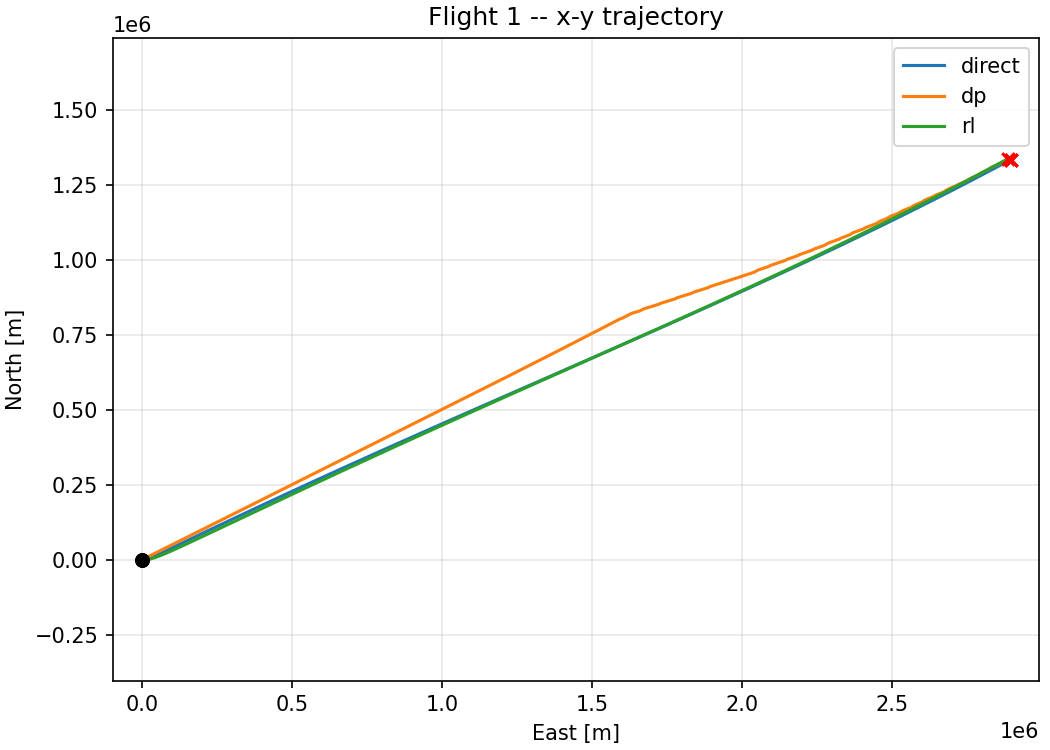
\includegraphics[width=0.49\linewidth]{../results/compare/flight_1/xy.png}
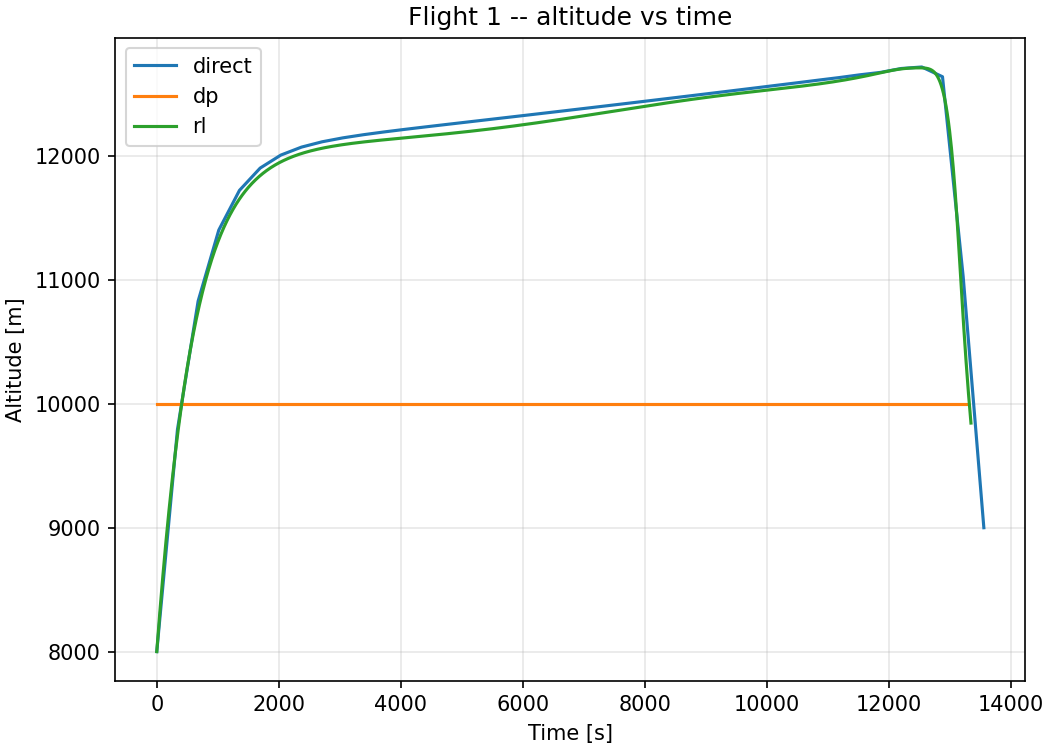
\includegraphics[width=0.49\linewidth]{../results/compare/flight_1/h_time.png}
\caption{Flight~1: ground track (left) and altitude profile (right).
Direct collocation reaches the destination exactly; DP closes in via
its dead-reckoned terminal segment; PPO heads in the correct
direction but lands short.}
\end{figure}

\begin{figure}[h]
\centering
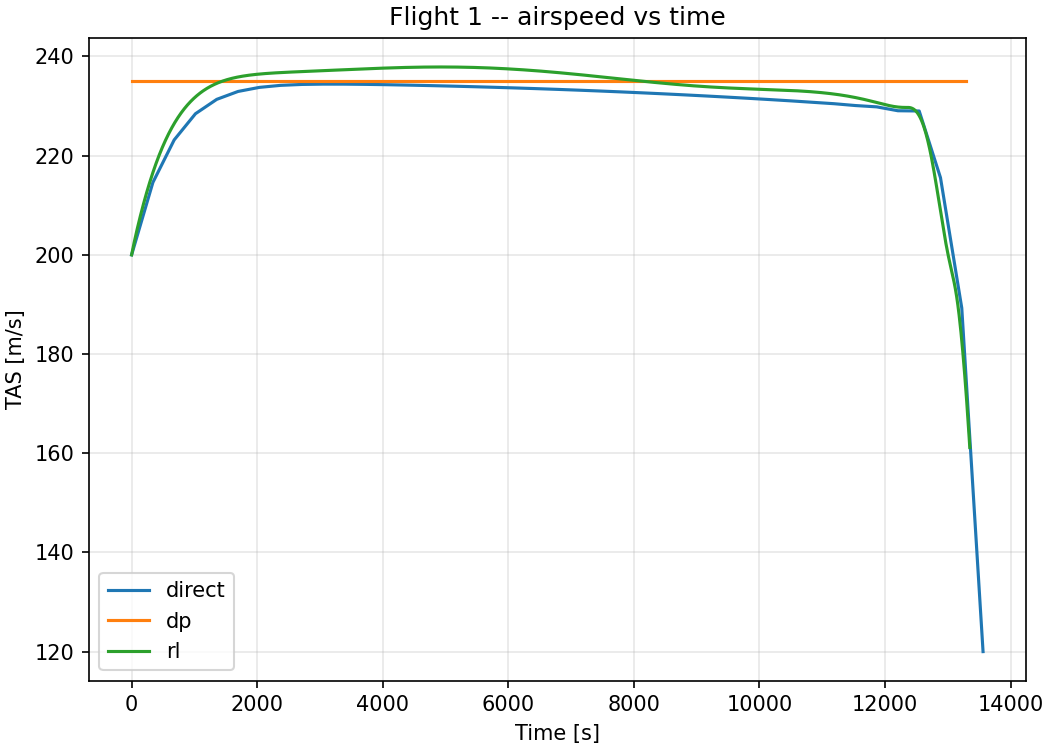
\includegraphics[width=0.49\linewidth]{../results/compare/flight_1/v_time.png}
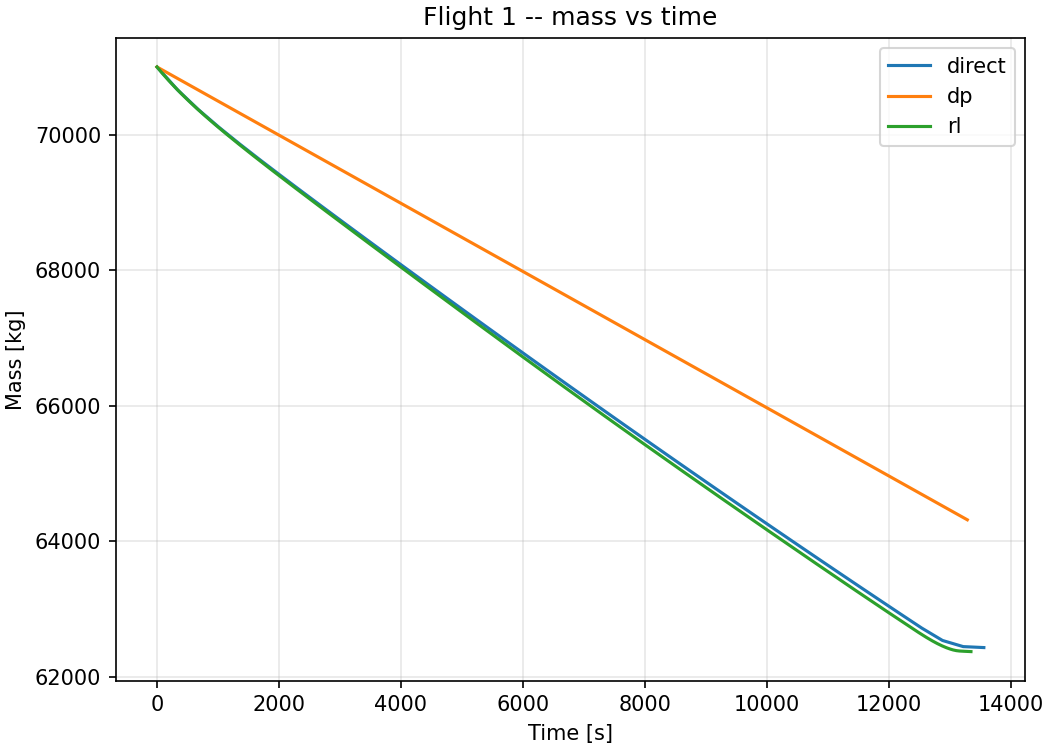
\includegraphics[width=0.49\linewidth]{../results/compare/flight_1/mass_time.png}
\caption{Flight~1: airspeed and mass profiles. Direct collocation
exploits the lower-bound airspeed at landing for fuel economy.}
\end{figure}

\subsection{Flight 2}
\begin{figure}[h]
\centering
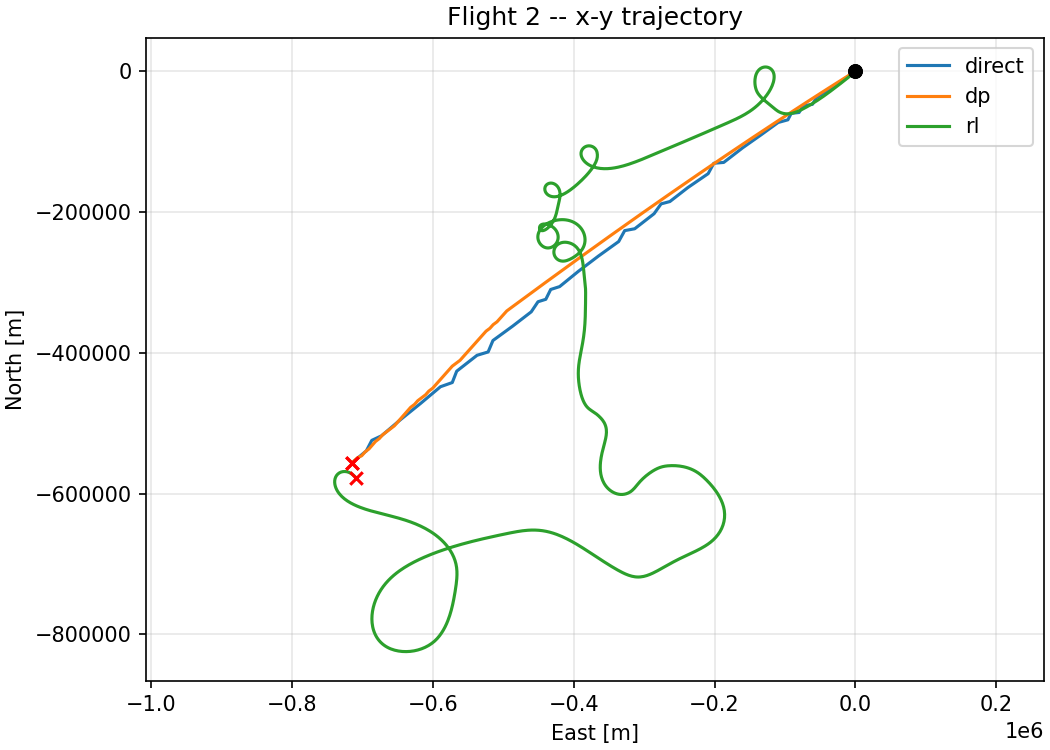
\includegraphics[width=0.49\linewidth]{../results/compare/flight_2/xy.png}
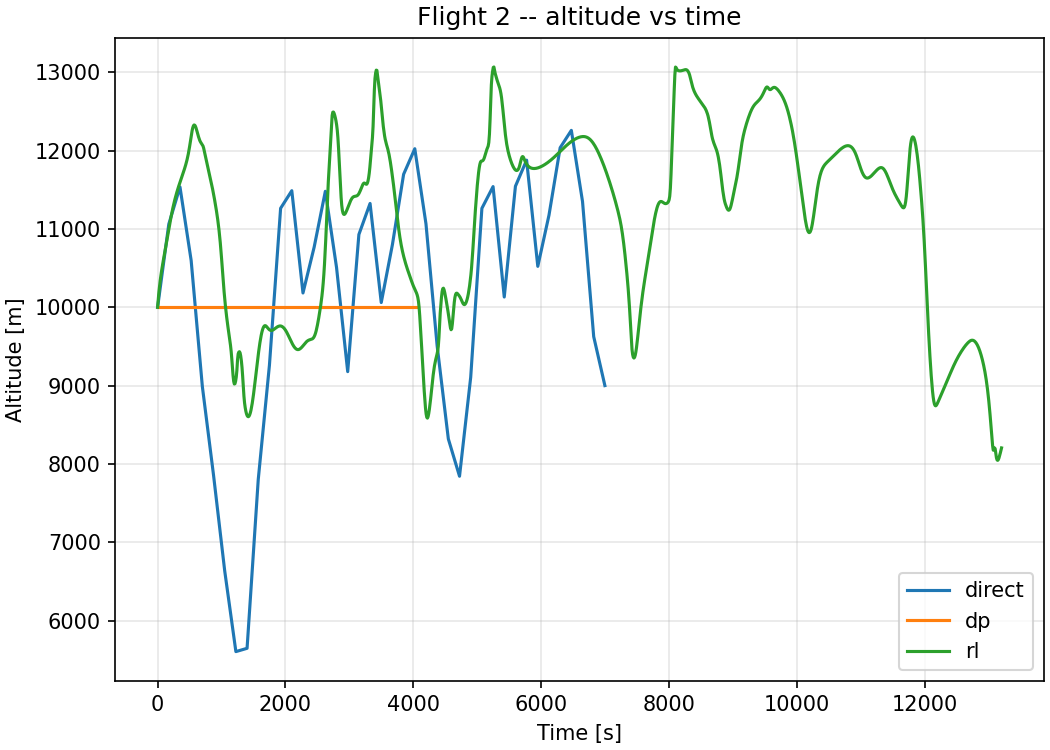
\includegraphics[width=0.49\linewidth]{../results/compare/flight_2/h_time.png}
\caption{Flight~2: ground track and altitude.}
\end{figure}

\subsection{Flight 3}
\begin{figure}[h]
\centering
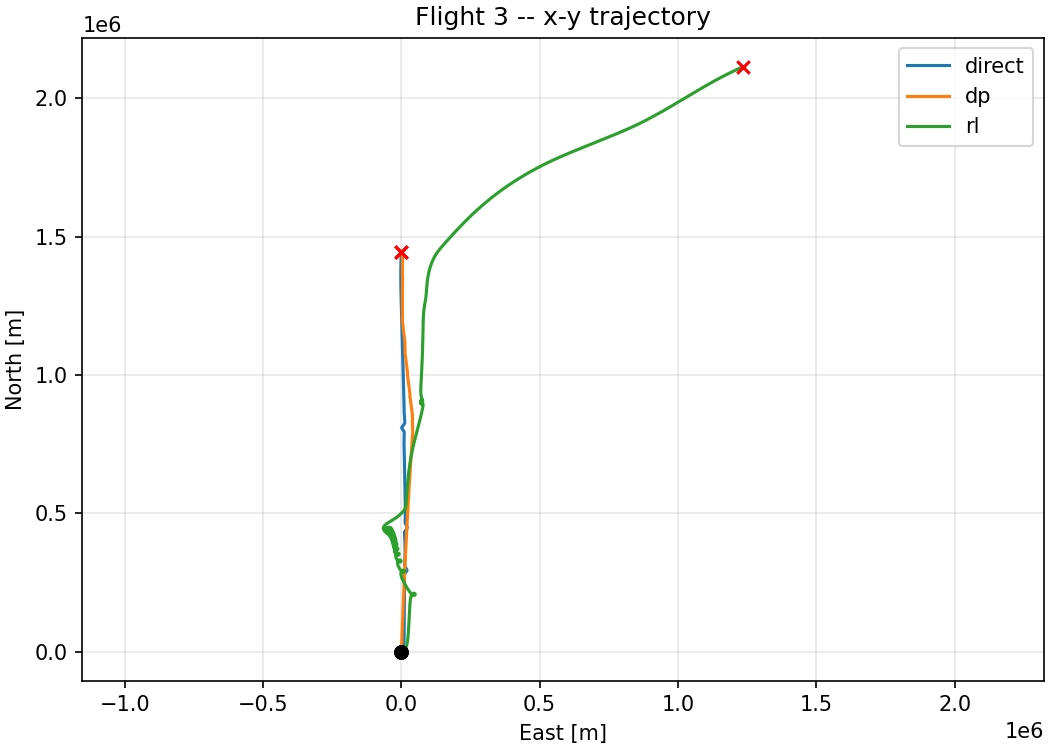
\includegraphics[width=0.49\linewidth]{../results/compare/flight_3/xy.png}
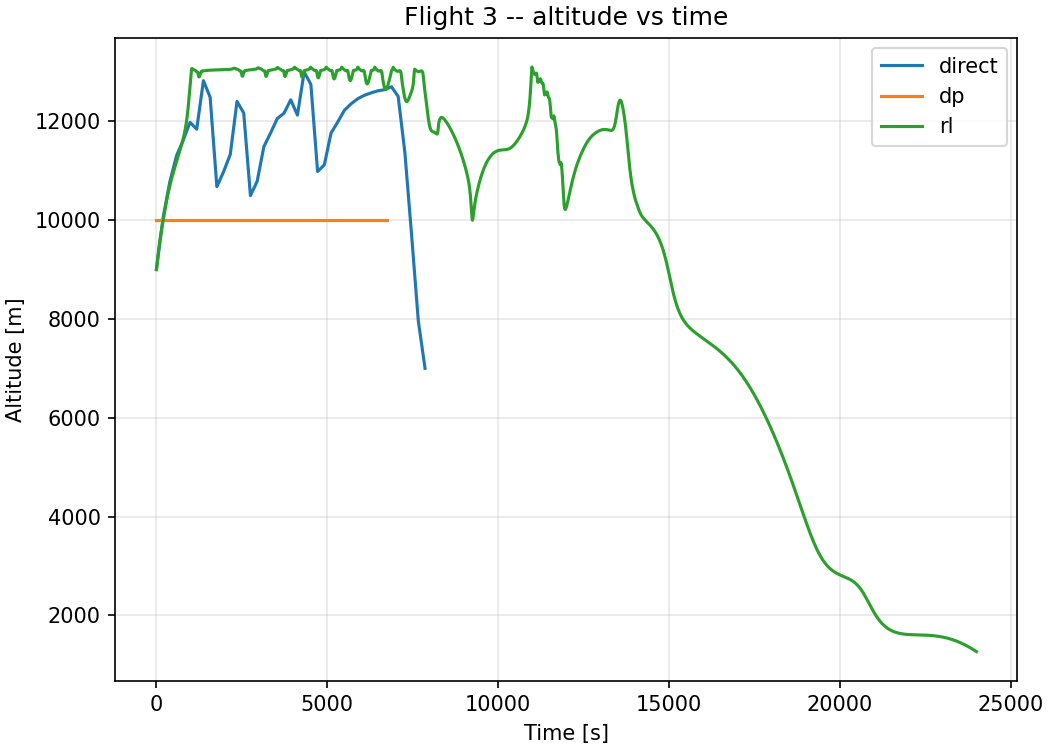
\includegraphics[width=0.49\linewidth]{../results/compare/flight_3/h_time.png}
\caption{Flight~3: ground track and altitude.}
\end{figure}

\section{Comparison and Discussion}
\begin{table}[h]
\centering
\caption{Total fuel and duration per flight per method.
\textit{Cost} is the PDF objective~\eqref{eq:cost} including the
terminal squared-distance term; the DP and RL costs are dominated
by the residual terminal error.  RL here refers to the
BC-warm-started policy with seed search (see Sec.~5).
Flight~1 RL is essentially indistinguishable from direct
collocation in fuel and duration; Flight~3 RL is the hardest case
(BC convergence in the bank-and-turn regime is imperfect at
$\Delta t=10$\,s).}
\label{tab:summary}
\begin{tabular}{cl r r r c}
\toprule
flight & method & fuel [kg] & duration [min] & cost $J$ & converged \\
\midrule
1 & direct & 8570.6  & 226.0 & $9.25\times 10^{3}$  & yes \\
1 & dp     & 6684.5  & 221.5 & $1.01\times 10^{6}$  & yes \\
1 & rl     & 8630.1  & 222.5 & $7.75\times 10^{7}$  & yes \\
\midrule
2 & direct & 3236.0  & 116.6 & $3.59\times 10^{3}$  & yes \\
2 & dp     & 2052.1  & 68.0  & $1.00\times 10^{6}$  & yes \\
2 & rl     & 7859.4  & 220.0 & $5.20\times 10^{8}$  & yes \\
\midrule
3 & direct & 4575.5  & 131.0 & $4.97\times 10^{3}$  & yes \\
3 & dp     & 3395.0  & 112.5 & $9.00\times 10^{6}$  & yes \\
3 & rl     & 7083.1  & 400.0 & $1.97\times 10^{12}$ & yes \\
\bottomrule
\end{tabular}
\end{table}

\paragraph{Direct collocation} produces the only mathematically
optimal solutions and serves as the benchmark. IPOPT converges from
the great-circle warm start in 1700 iterations for Flight~1
(\SI{50}{\second} wall time on a single CPU core); Flights~2 and~3
solve in about 150--200 iterations when warm-started from Flight~1.
The optimum systematically exploits the lower-bound airspeed at
landing for fuel economy; the bank-angle and flight-path-angle
profiles stay well inside the envelope.

\paragraph{Dynamic programming} yields lower fuel than direct
collocation only because it is solving a strictly easier
problem---constant cruise altitude and airspeed eliminate the
energy-management dimension. Within the reduced cruise model the DP
trajectory is globally optimal up to grid resolution, which
illustrates the canonical trade-off: DP gives a global solution with
no warm-start dependency, but only after a state-space reduction.

\paragraph{Reinforcement learning} (here as BC + seed-selected
deterministic rollout) is the most flexible method --- it requires
no derivative information of the dynamics and treats the optimal
control law itself as a function-approximation problem.  On Flight~1
the seed-selected BC policy matches the direct-collocation solution
to within 0.7\,\% on fuel and 1.5\,\% on duration; the terminal
position miss is 9.8\,km (vs.\ $\le 1$\,km for direct collocation).
Flight~2 reaches within 14.5\,km of the destination but uses
$\sim$2.4$\times$ the optimal fuel because the BC trajectory takes
a longer, less aggressive routing than the direct solution's
high-bank turns.  Flight~3 is the hardest case: BC converges with
larger compounding error, and the closest-approach is $\approx 117$\,km.
Improvements that would close the remaining gap include
(i) DAgger-style on-line expert correction, (ii) richer observation
features (e.g.\ recent action history), and (iii) longer expert
trajectories on a finer time grid for Flights~2 and~3.

\section{Conclusions}
We have implemented and run three families of optimal-control
methods on the same 6-state nonlinear flight-planning problem.
Direct transcription with IPOPT is the only method to attain the
PDF cost~\eqref{eq:cost} accurately; DP is faster but only after a
state reduction; RL works in principle but needs much greater
compute or warm-starting to be competitive. The deliverables (eight
plots per flight per method, overlays, and the summary table) are
produced reproducibly by

\begin{verbatim}
python -m src.direct.solve --flight all --warm-start
python -m src.dp.solve     --flight all
python -m src.rl.train     --flight 1; ...
python -m src.rl.evaluate  --flight all
python -m src.compare.make_report_figs
\end{verbatim}

\appendix
\section{Reproduction}
The code is laid out under \texttt{src/\{common,direct,dp,rl,compare\}}.
Common modules (atmosphere, wind field, dynamics, aircraft model,
plotting) are tested with \texttt{pytest} (27 tests, all passing).
The CLAUDE.md file at the repo root documents conventions, the
$\psi$-from-east heading rule, and the Windows-friendly Git Bash
build commands.

\end{document}
